\ifdefined\COMPLETE
\else
    \input{./preambule-sacha-utf8.ltx}
    \begin{document}
\fi

                 
                 \intitule{Calcul fractionnaire : cours} 
                 
\tikzstyle{operation}=[<-,>=latex]   
\tikzstyle{etiquette}=[midway,fill=black!20]        
      
\begin{flushright}
\begin{tikzpicture}
\node (f) at (0,0)  {\Large $\dfrac{a}{b}$};
\node (n) at (2,.75) {numérateur} ; 
\node (d) at (2,-.75) {dénominateur} ;  
\draw[operation] (f) to[out=50,in=180] node[left] {} (n);
\draw[operation] (f) to[out=-50,in=180] node[left] {} (d);
\end{tikzpicture}
\end{flushright}

\vspace*{-2.5cm}
\renewcommand{\labelitemi}{\textbullet}
    
\Asavoir{\underline{{\large 1)} Addition}} 
\begin{itemize}
\item On met les deux fractions au même dénominateur ;
\item On ajoute les numérateurs.
\end{itemize}

\bigskip   

\Asavoir{\underline{{\large 2)} Soustraction}} 
\begin{itemize}
\item On met les deux fractions au même dénominateur ;
\item On soustraie les numérateurs.
\end{itemize}

\bigskip   

\Asavoir{\underline{{\large 3)} Multiplication}} 
\begin{itemize}
\item On regarde si on peut simplifier l'une ou l'autre des deux fractions\\
      dans ce cas on simplifie;
\item On multiplie les numérateurs et les dénominateurs entre-eux ; 
\item On regarde si on peut simplifier la fraction obtenue\\
      Si oui, on simplifie.
\end{itemize}

\bigskip   

\Asavoir{\underline{{\large 4)}Division}} 
\begin{itemize}
\item On transforme la seconde fraction en son inverse
      et la division par une multiplication ;
\item On applique la méthode de la multiplication {\large \ding{174}} .
\end{itemize}

\bigskip

\bigskip 
                   
%                 \intitule{Calcul fractionnaire} 

                 \centerline{\intitule{Exemples rédigés de quatre types}}   

\bigskip                     
                 
\Asavoir{{\large 1) }\underline{Addition}}  

\begin{tikzpicture}
\node (a) at (-.75,4.5)  {$\dfrac{1}{2} + \dfrac{3}{5}$};
\node at (0,4.5)  {$=$};
\node (b) at (4.2,4.5)  {$\dfrac{1\textcolor{red}{\times 5}}{2\textcolor{red}{\times 5}} + \dfrac{3\textcolor{red}{\times 2}}{5\textcolor{red}{\times 2}} \qquad$ \methode {On met au même dénominateur}};
\node  at (0, 3.5) { $=$} ; 
\node (c) at (1.2, 3.5) {$\dfrac{5}{10} + \dfrac{6}{10}$ }; 
\node  at (0, 2.5) { $=$} ; 
\node (d) at (1.2, 2.5) {$\dfrac{11}{10}$ }; 
\draw[color=blue,->,>=latex] (c) to[out=0,in=0]
node[midway,right]{\methode{\hspace*{.65cm}  On ajoute les numérateurs}} (d);
\end{tikzpicture}

\bigskip                     
                
\bigskip                     
                  
\Asavoir{{\large 2) }\underline{Soustraction}}  

\begin{tikzpicture}
\node (a) at (-.75,4.5)  {$\dfrac{4}{7} - \dfrac{2}{3}$};
\node at (0,4.5)  {$=$};
\node (b) at (4.2,4.5)  {$\dfrac{4\textcolor{red}{\times 3}}{7\textcolor{red}{\times 3}} + \dfrac{2\textcolor{red}{\times 7}}{3\textcolor{red}{\times 7}} \qquad$ \methode {On met au même dénominateur}};
\node  at (0, 3.5) { $=$} ; 
\node (c) at (1.2, 3.5) {$\dfrac{12}{21} - \dfrac{14}{21}$ }; 
\node  at (0, 2.5) { $=$} ; 
\node (d) at (1.2, 2.5) {$-\dfrac{2}{21}$ }; 
\draw[color=blue,->,>=latex] (c) to[out=0,in=0]
node[midway,right]{\methode{\hspace*{.65cm}On soustraie les numérateurs}} (d);
\end{tikzpicture}

\newpage 

\Asavoir{{\large 3) }\underline{Multiplication}}  

\setbox1=\vtop{ \hsize=5cm \null % null assure l'alignement par le haut 
\begin{tikzpicture}% [every node/.style={anchor=west}]
  \matrix (m) [matrix of math nodes,
row sep=0cm,column sep=0cm,  
% nodes={rectangle, draw},  
%    nodes in empty cells,
column 1/.style={anchor=base east},
column 3/.style={anchor=base west}]{
\dfrac{4}{6} \times \dfrac{1}{8}
     &=& 
         |(a)|  \dfrac{2\textcolor{red}{\times 2}}{3\textcolor{red}{\times 2}} \times \dfrac{1}{8}  \\
     &=&  
         |(b)| \dfrac{2}{3} \times \dfrac{1}{8}  \\ 
     &=& |(d)| \dfrac{2 \times 1}{3 \times 8} \\
     &=& |(e)| \dfrac{2}{24} \\
     &=& |(g)| \dfrac{2 \times 1}{2 \times 12} \\
     &=& |(h)| \dfrac{1}{12} \\
};   
\node [right = 0.1 cm of b.east] (c) {} ; 
\draw[color=blue,->,>=latex] (a) to[out=0,in=0]
   node[midway,right]{\hspace*{.65cm}\methode{On simplifie $\dfrac{4}{6}=\dfrac{2}{3}$}} (c);  
\node [right = 0.1 cm of e.east] (f) {} ; 
\draw[color=blue,->,>=latex] (d) to[out=0,in=0]
   node[midway,right]{
   \hspace*{.65cm}\methode{\hspace*{.5cm}\methode{ \begin{minipage}[c]{.46\linewidth}
      On multiplie les numérateurs\\ 
      et les dénominateurs entre eux
   \end{minipage}}}
   } (f);                 
\node [right = 0.1 cm of h.east] (i) {} ; 
\draw[color=blue,->,>=latex] (g) to[out=0,in=0]
   node[midway,right]{\hspace*{1cm}\methode{On simplifie $\dfrac{2}{24}=\dfrac{1}{12}$}} (i);  
\node [right = 0.1 cm of e.east] (f) {} ;    
\end{tikzpicture}}

\box1

\bigskip                     
           

\bigskip                     
                                  
\Asavoir{{\large 4) }\underline{Division}}  


\setbox1=\vtop{ \hsize=5cm \null % null assure l'alignement par le haut 
\begin{tikzpicture}% [every node/.style={anchor=west}]
  \matrix (m) [matrix of math nodes,
row sep=0cm,column sep=0cm,  
% nodes={rectangle, draw},  
%    nodes in empty cells,
column 1/.style={anchor=base east},
column 3/.style={anchor=base west}]{
\displaystyle { % eloigne les deux fractions
                           \; \dfrac{1}{8} \; 
                             \over 
                           \; \dfrac{4}{6} \;
                           }
     &=& 
         |(a)|  \dfrac{1}{8} \div \dfrac{6}{4} = \dfrac{1}{8} \times \dfrac{4}{6} \\
     &=&  
         |(b)| \dfrac{1}{8} \times \dfrac{2}{3}  
                 & |(l)|\text{\hspace*{1cm}\methode{On simplifie}} \\ 
     &=& |(d)| \dfrac{2 \times 1}{3 \times 8} 
                 & \text{\hspace*{1cm}\methode{On multiplie}}  \\
     &=& |(h)| \dfrac{1}{12} 
                 & |(m)|\text{\hspace*{1cm}\methode{On simplifie}} \\
};   
 
\node [right = 1 cm of b.east] (c) {} ; 
\draw[color=blue,->,>=latex] (a) to[out=0,in=0]
   node[midway,right]{\hspace*{.5cm}{
   \methode{ \begin{minipage}[c]{.46\linewidth}
      On transforme en multiplication\\ 
      par l'inverse
   \end{minipage}}}
} (c);    
\node [right = .5 cm of b.east] (i) {} ; 
\node [right = .2 cm of d.east] (j) {} ; 
\draw[color=blue,->,>=latex] (i) to[out=0,in=0] (j);             
\draw[color=blue,->,>=latex] (d.east) to[out=0,in=0] (h);  
\node [right = 1 cm of l.east] (n) {} ; 
\node [right = 1 cm of m.east] (o) {} ; 
\draw[color=white] (n)-- 
node[midway,right]{\hspace*{.65cm}\methode{\begin{minipage}[c]{.46\linewidth}
      $\left\} \begin{matrix}
                              \\
                              \\
                              \mathrm{cf}\;\text{\large \ding{174}} \\
                              \\
                              \\
                      \end{matrix} \right.$
   \end{minipage}
}} (o);      
\end{tikzpicture}}

\box1
\ifdefined\COMPLETE
\else
    \end{document}
\fi